% SC4012 --- Chapter 2: Memory Safety (0->100 ground-up)
\chapter{Memory Safety: Stack Overflows, ROP, ASLR and CFI}
\label{ch:memory}

\begin{quote}
\emph{``Memory corruption is the original sin of C.''} --- Every unchecked copy, every dangling pointer, is a chance for data to become control. We see why, how it is exploited, and how modern defences raise the bar.
\end{quote}

\noindent\fbox{\parbox{\dimexpr\linewidth-2\fboxsep-2\fboxrule}{%
\textbf{From zero: how programs use memory.} We assume no systems background. We build from the stack layout (what a function call keeps), what ``overflowing'' means, and why overwriting a return address gives control. Every exploit is shown as picture $\to$ input bytes $\to$ hardening.}}
\vspace{0.4em}

\section*{Learning Outcomes}
After this chapter you will be able to:
\begin{enumerate}[label=(L\arabic*)]
    \item explain stack frames (buffers, saved \texttt{ebp}, return address) and why a buffer overflow corrupts control data;
    \item craft a minimal stack-overflow payload and explain ROP chaining;
    \item describe ASLR, stack canaries, DEP/W$\oplus$X and what each blocks;
    \item explain Control-Flow Integrity (CFI) and its forward/backward variants;
    \item select safe APIs and compiler flags that prevent or detect overflows.
\end{enumerate}

% ============================================================
\section{How the Stack Works}
\label{sec:stack-model}
Every function call reserves a \emph{frame} on the call stack: local buffers at low addresses, then the saved frame pointer, then the return address, then arguments of the caller. The stack grows toward lower addresses but buffers fill upward---toward control data. A copy that writes past the buffer inevitably reaches what determines ``where to return.''

\begin{definition}[Stack frame]
On x86/x64 the frame for \texttt{f} contains (low $\to$ high): local variables (e.g., \texttt{char buf[64]}), saved \texttt{ebp/rbp}, return address, and caller data. The CPU register \texttt{esp/rsp} points to the top; \texttt{ret} pops the return address into \texttt{eip/rip}.
\end{definition}

\begin{figure}[h]\centering
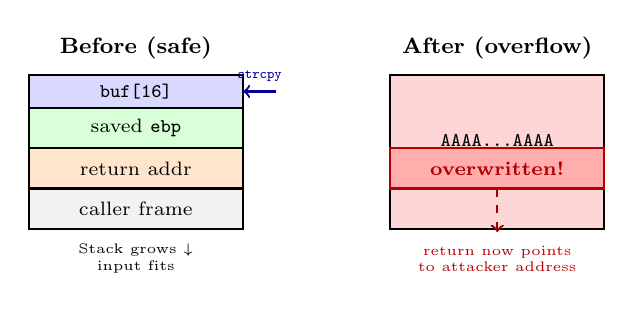
\begin{tikzpicture}[scale=0.85,every node/.style={font=\scriptsize}]
  % safe
  \node[font=\footnotesize\bfseries] at (1.6,3.9) {Before (safe)};
  \draw[thick,fill=blue!15] (0,3.0) rectangle (3.2,3.5) node[midway] {\texttt{buf[16]}};
  \draw[thick,fill=green!15] (0,2.4) rectangle (3.2,3.0) node[midway] {saved \texttt{ebp}};
  \draw[thick,fill=orange!20] (0,1.8) rectangle (3.2,2.4) node[midway] {return addr};
  \draw[thick,fill=gray!10] (0,1.2) rectangle (3.2,1.8) node[midway] {caller frame};
  \draw[->,thick,blue!60!black] (3.7,3.25) -- (3.2,3.25) node[midway,above,font=\tiny] {\texttt{strcpy}};
  \node[font=\tiny,align=center] at (1.6,0.75) {Stack grows $\downarrow$\\input fits};
  % overflowed
  \node[font=\footnotesize\bfseries] at (7.0,3.9) {After (overflow)};
  \draw[thick,fill=red!16] (5.4,1.2) rectangle (8.6,3.5) node[midway,align=center] {\texttt{AAAA...AAAA}\\ \texttt{+\;0x0804861a}};
  \draw[thick,fill=red!32,draw=red!70!black] (5.4,1.8) rectangle (8.6,2.4) node[midway,font=\scriptsize\bfseries,text=red!70!black] {overwritten!};
  \node[font=\tiny,align=center,red!70!black] at (7.0,0.75) {return now points\\to attacker address};
  \draw[->,thick,dashed,red!60!black] (7.0,1.8) -- (7.0,1.15);
\end{tikzpicture}
\caption{Stack frame before and after an overflow. An unchecked 28-byte write into a 16-byte buffer spills over the saved frame pointer and return address (red). On \texttt{ret} the CPU jumps to the attacker's address.}
\label{fig:stack-overflow2}
\end{figure}

\begin{lstlisting}[language=C]
#include <string.h>
#include <stdio.h>
void vulnerable(char *input) {
    char buf[16];
    strcpy(buf, input);   // no bounds check -- NEVER use
    printf("echo: %s\n", buf);
}
int main(int argc, char **argv){
    if(argc>1) vulnerable(argv[1]);
    return 0;
}
\end{lstlisting}
Supplying 20~`A's plus \texttt{\textbackslash x1a\textbackslash x86\textbackslash x04\textbackslash x08} overwrites the 4-byte return address with \texttt{0x0804861a}. With DEP off, that address could point into shellcode placed in \texttt{buf}; with DEP on, it points to a code gadget (next).

\begin{example}[Off-by-one and why size matters]
\texttt{for(i=0;i<=16;i++) buf[i]=input[i];} writes 17 bytes into \texttt{buf[16]} (indices $0$--$15$ are valid). The extra byte corrupts the saved \texttt{ebp} LSB, shifting the next frame. On 64-bit, addresses are 8 bytes and a canary sits before the return address, so more bytes and a leak are needed, but the geometry is identical.
\end{example}

% ============================================================
\section{From Shellcode to ROP}
\label{sec:rop}
\emph{Shellcode injection} places machine bytes in the buffer and jumps to them. Write-XOR-Execute (W$\oplus$X / DEP) marks data pages non-executable, so the CPU faults if it fetches from the stack. Attackers adapted: instead of injecting code, chain snippets of \emph{existing} executable code ending in \texttt{ret}.

\begin{definition}[ROP gadget and chain]
A \emph{gadget} is a short instruction sequence in executable memory ending in \texttt{ret} (e.g., \texttt{pop eax; ret}). A \emph{ROP chain} is a sequence of gadget addresses placed on the stack so each \texttt{ret} jumps to the next gadget, achieving arbitrary computation without injecting code (Turing-complete given enough gadgets).
\end{definition}

\begin{figure}[h]\centering
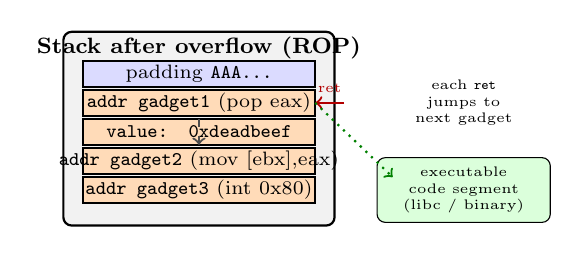
\begin{tikzpicture}[scale=0.82,every node/.style={font=\scriptsize}]
  \draw[thick,fill=gray!10,rounded corners=3pt] (0,0) rectangle (4.2,3.0);
  \node[font=\footnotesize\bfseries] at (2.1,2.75) {Stack after overflow (ROP)};
  \draw[thick,fill=blue!14] (0.3,2.15) rectangle (3.9,2.55) node[midway] {padding \texttt{AAA...}};
  \draw[thick,fill=orange!28] (0.3,1.70) rectangle (3.9,2.10) node[midway] {\texttt{addr gadget1} (pop eax)};
  \draw[thick,fill=orange!28] (0.3,1.25) rectangle (3.9,1.65) node[midway] {\texttt{value: 0xdeadbeef}};
  \draw[thick,fill=orange!28] (0.3,0.80) rectangle (3.9,1.20) node[midway] {\texttt{addr gadget2} (mov [ebx],eax)};
  \draw[thick,fill=orange!28] (0.3,0.35) rectangle (3.9,0.75) node[midway] {\texttt{addr gadget3} (int 0x80)};
  \draw[->,thick,red!70!black] (4.35,1.90) -- (3.9,1.90) node[midway,above,font=\tiny] {ret};
  \draw[->,thick,gray!60!black,dashed] (2.1,1.65) -- (2.1,1.25);
  \node[font=\tiny,align=center] at (6.2,1.90) {each \texttt{ret}\\jumps to\\next gadget};
  \node[draw,fill=green!14,rounded corners=3pt,minimum width=2.2cm,align=center,font=\tiny] at (6.2,0.55) {executable\\code segment\\(libc / binary)};
  \draw[->,thick,green!50!black,dotted] (3.9,1.90) -- (5.1,0.75);
\end{tikzpicture}
\caption{ROP chain on the stack. The overwritten return address points to gadget1; each gadget's trailing \texttt{ret} pops the next address from the stack. No injected code is executed.}
\label{fig:rop-chain}
\end{figure}

Scarcity is not a defence: large binaries and \texttt{libc} contain thousands of gadgets; automated tools (ROPgadget, ropper) find them. The fix is not ``fewer gadgets'' but making addresses unpredictable (ASLR) and control flow unforgeable (CFI).

% ============================================================
\section{Hardening: Canaries, ASLR, DEP, and CFI}
\label{sec:hardening-mem}
No single layer suffices; they compose. Each blocks a different stage.

\begin{figure}[h]\centering
\resizebox{\linewidth}{!}{%
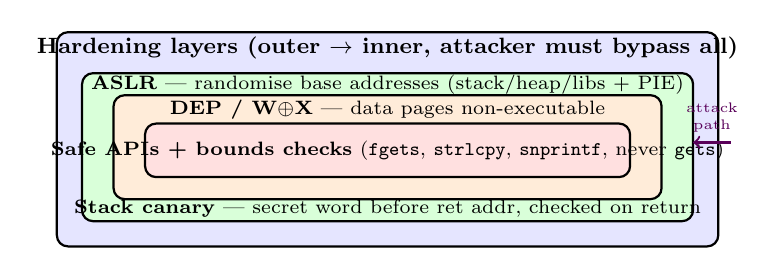
\begin{tikzpicture}[scale=0.80,every node/.style={font=\scriptsize}]
  \draw[thick,fill=blue!10,rounded corners] (0,0) rectangle (10.5,3.4);
  \node[font=\footnotesize\bfseries] at (5.25,3.15) {Hardening layers (outer $\to$ inner, attacker must bypass all)};
  \draw[thick,fill=green!15,rounded corners] (0.4,0.4) rectangle (10.1,2.75);
  \draw[thick,fill=orange!15,rounded corners] (0.9,0.75) rectangle (9.6,2.40);
  \draw[thick,fill=red!12,rounded corners] (1.4,1.10) rectangle (9.1,1.95);
  \node[align=center] at (5.25,1.52) {\textbf{Safe APIs + bounds checks} (\texttt{fgets}, \texttt{strlcpy}, \texttt{snprintf}, never \texttt{gets})};
  \node[align=center] at (5.25,2.17) {\textbf{DEP / W$\oplus$X} --- data pages non-executable};
  \node[align=center] at (5.25,2.57) {\textbf{ASLR} --- randomise base addresses (stack/heap/libs + PIE)};
  \node[align=center] at (5.25,0.60) {\textbf{Stack canary} --- secret word before ret addr, checked on return};
  \draw[->,thick,violet!70!black] (10.7,1.65) -- (10.1,1.65) node[midway,above,font=\tiny,align=center] {attack\\path};
\end{tikzpicture}}%
\caption{Defence in depth for memory corruption. Input validation stops malformed data earliest; DEP stops execution of injected code; ASLR hides gadget addresses; canary detects linear overflows. CFI (not shown) constrains which indirect targets are legal.}
\label{fig:hardening-layers-mem}
\end{figure}

\begin{description}[leftmargin=1.2em,itemsep=0.35em]
    \item[Stack canaries] Compiler inserts a random word between \texttt{buf} and the return address; on return it is checked, mismatch calls \texttt{\_\_stack\_chk\_fail}. Bypass requires leaking the canary, corrupting a function pointer \emph{before} it, or a non-linear write.
    \item[ASLR] Randomises bases of stack, heap and libraries per run; with PIE, the executable too. 32-bit offers only $8$--$16$ bits of entropy (brute-forceable); 64-bit offers $28$+ bits. Bypass needs an information leak (format string, over-read) that reveals a pointer.
    \item[DEP/W$\oplus$X] NX bit marks stack/heap non-executable; injected shellcode faults. Bypass via ROP/JOP.
    \item[CFI] Compiler instruments every indirect call/jump/return to check the target belongs to a precomputed control-flow graph. Forward-edge CFI guards calls through function pointers; backward-edge CFI (shadow stack) guards returns. Even with a leak and ROP gadgets, only CFG-legal targets are allowed, breaking chains.
\end{description}

\begin{figure}[h]\centering
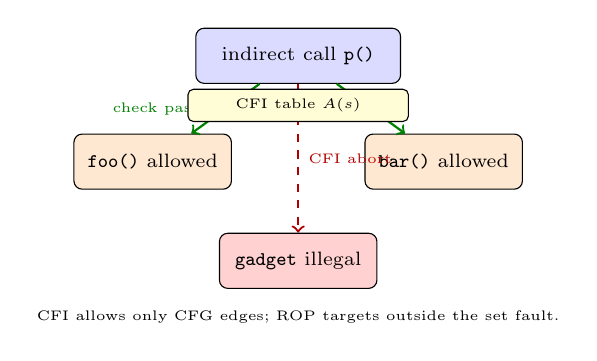
\begin{tikzpicture}[scale=0.84,every node/.style={font=\scriptsize}]
  \node[draw,fill=blue!14,rounded corners=3pt,minimum width=2.6cm,minimum height=0.7cm,align=center] (call) at (0,1.6) {indirect call \texttt{p()}};
  \node[draw,fill=orange!18,rounded corners=3pt,minimum width=2.0cm,minimum height=0.7cm,align=center] (ok1) at (-2.2,0) {\texttt{foo()} allowed};
  \node[draw,fill=orange!18,rounded corners=3pt,minimum width=2.0cm,minimum height=0.7cm,align=center] (ok2) at (2.2,0) {\texttt{bar()} allowed};
  \node[draw,fill=red!18,rounded corners=3pt,minimum width=2.0cm,minimum height=0.7cm,align=center] (bad) at (0,-1.5) {\texttt{gadget} illegal};
  \draw[->,thick,green!50!black] (call) -- (ok1) node[midway,left,font=\tiny] {check passes};
  \draw[->,thick,green!50!black] (call) -- (ok2);
  \draw[->,thick,red!70!black,dashed] (call) -- (bad) node[midway,right,font=\tiny] {CFI abort};
  \node[draw,fill=yellow!16,rounded corners=2pt,minimum width=2.8cm,align=center,font=\tiny] at (0,0.85) {CFI table $A(s)$};
  \node[font=\tiny,align=center] at (0,-2.35) {CFI allows only CFG edges; ROP targets outside the set fault.};
\end{tikzpicture}
\caption{Forward-edge CFI. The call site $s$ may target only the precomputed allowed set $A(s)$; any other address (e.g., a gadget) is rejected even if the attacker controls the pointer.}
\label{fig:cfi}
\end{figure}

\begin{definition}[CFI guarantee]
If the program's CFG is sound, CFI ensures every indirect control transfer at runtime follows an edge in the CFG. Formally, for indirect call site $s$ with allowed set $A(s)$, the check $target\in A(s)$ is enforced; on failure the process aborts. Precision of $A(s)$ determines security vs.\ compatibility.
\end{definition}

Composition matters: canary catches linear overflows but not a heap vtable overwrite before it; ASLR hides addresses but not if a single leak reveals them; DEP stops shellcode but not ROP; CFI restricts targets but needs a precise CFG (over-approximation re-enables gadgets). Real exploits chain a leak to defeat ASLR, a ROP chain to defeat DEP, and a non-linear write or stolen canary to defeat the cookie. That is why the checklist is a conjunction, not a menu.

\begin{remark}[Why memory safety is a language problem]
Bounds checking every access in software costs $5$--$20\times$ slowdown if naïve. Memory-safe languages (Rust's ownership, Go's GC, Java's array checks) enforce it by construction; hardware (ARM MTE tags memory, Intel MPX/CET) accelerates it. The long-term fix is to not write new C for untrusted input, and to sandbox legacy C (seccomp, pledge) so a single overflow does not equal full compromise. Fuzzing (Ch.~5) and verification (Ch.~6) catch bugs that remain.
\end{remark}

Compilation checklist: \texttt{-fstack-protector-strong -D\_FORTIFY\_SOURCE=2 -Wl,-z,RelRO,-z,Now -fPIE -pie} plus runtime ASLR (\texttt{/proc/sys/kernel/randomize\_va\_space=2}). For new code, prefer memory-safe languages (Rust, Go) or hardware assistance (ARM MTE, Intel CET).

\begin{lstlisting}[language=C]
// Safe alternatives: always bound the copy
char buf[16];
if (fgets(buf, sizeof(buf), stdin) == NULL) handle_error();
// or strlcpy / snprintf with explicit size; never gets/strcpy on untrusted input
// With _FORTIFY_SOURCE, strcpy into a known-size object is checked at runtime.
\end{lstlisting}

% ============================================================
\section{Why Defences Must Compose}
\label{sec:compose-mem}
A single bug should not be a single exploit. The composition argument is: Safe APIs remove the bug; if a bug remains, the canary detects the spill; if the canary is bypassed (non-linear write), ASLR forces the attacker to also obtain a leak; if a leak is obtained, DEP still blocks injected code; if ROP bypasses DEP, CFI still restricts targets. Each layer requires a distinct primitive (overflow, leak, write, execute), so an attacker needs a chain of bugs, not one.

Quantitatively, 32-bit ASLR with 8 bits of entropy is bypassed in $2^{7}=128$ tries on average (feasible); 64-bit with 28 bits needs $2^{27}$ tries (infeasible without a leak). Canaries are 32--64 random bits; guessing is infeasible, but a format-string leak or a byte-by-byte brute force fork (e.g., forking server) can disclose them. This guides prioritisation: fix leaks first, then enable the full stack.

% ============================================================
\section{Heap, Use-After-Free and Format Strings}
\label{sec:heap-uaf}
Stack is not the only target. Heap overflows corrupt allocator metadata or adjacent objects (C++ vtables, function pointers in structs). Use-after-free (UAF) keeps a dangling pointer after \texttt{free}; reallocation may place attacker-controlled data where the program still trusts a vtable. Format-string bugs (\texttt{printf(user\_input)}) give both a leak (\texttt{\%p \%x}) and a write (\texttt{\%n}), defeating ASLR and canaries in one primitive.

\begin{lstlisting}[language=C]
// Format-string leak + write (DO NOT DO THIS)
char *user = get_input();
printf(user);  // vulnerable: user controls format string
// attacker input "%p.%p.%n" leaks stack words then writes to a pointer
// Fix: printf("%s", user);
\end{lstlisting}

The principle is unchanged: data reaches control. Modern allocators add safe unlinking, heap canaries, and isolated heaps; sanitizers (ASan) detect UAF and overflows at runtime; fuzzing (Ch.~5) finds them before attackers do.

% ============================================================
\section{Exercises}
\label{sec:ch02-exercises}
% Exercises with sloppy for long \texttt lines
{\sloppy
\begin{enumerate}[label=E2.\arabic*, leftmargin=*, itemsep=0.6em]
    \item \textbf{Stack arithmetic.} \texttt{char buf[16];} then 4~B canary, 4~B saved \texttt{ebp}, 4~B return address on 32-bit. How many bytes to overwrite the canary? The return address? If the canary is 4 random bytes with a zero byte, why does \texttt{strcpy} make brute force harder?
    \item \textbf{ROP chain sketch.} Gadgets: \texttt{(a) pop eax; ret}, \texttt{(b) pop ebx; ret}, \texttt{(c) mov [ebx],eax; ret}, \texttt{(d) int 0x80; ret}. Show stack contents that write \texttt{0xdeadbeef} to address \texttt{0x0804a100} using (a)--(c). What extra gadget would you need to invoke \texttt{execve}?
    \item \textbf{Bypassing layers.} Explain why DEP alone does not stop ROP and why ASLR alone fails if the attacker has a format-string leak (\texttt{printf(user\_input)}). Describe a two-stage leak$\to$ROP bypass of DEP+ASLR and which layer (canary or CFI) blocks it earliest.
    \item \textbf{CFI precision.} A call site \texttt{void (*p)(int)} has static type ``function taking int.'' Forward CFI allows any function with that type. Give an example where this still permits an exploit (type-collision) and how shadow stacks or finer CFI would stop it.
    \item \textbf{Safe-code audit.} Audit: \texttt{char dst[32];} \texttt{strcpy(dst, getenv(\"HOME\"));} \texttt{sprintf(buf,\"\%s/\%s\",dir,file);}. List the overflows and rewrite with \texttt{snprintf}/\texttt{strlcpy} and explicit length checks, handling truncation as error.
\end{enumerate}
\par}

\section*{Chapter Notes}
Aleph One, ``Smashing the Stack for Fun and Profit'' (Phrack~49, 1996) is the canonical overflow note; ``SoK: Eternal War in Memory'' (Szekeres et al., Oakland~2013) surveys defences. ROP is from Shacham (CCS~2007); JOP from Bletsch et al. ASLR details in PaX; canaries in StackGuard/ProPolice. CFI from Abadi et al. (CCS~2005); modern realisations include LLVM-CFI and Intel CET / ARM BTI/PAC. Memory-safe languages and MTE/CET are the forward path.

% End of Chapter 2
